\section{Introduction}\label{sec:intro}

A ball falls through a Galton board with $N$ rows of pegs. At the first peg it
goes left or right with probability $\frac12$. At every later peg it repeats
its previous direction with probability $p$ and switches with probability
$q=1-p$. Problem~131 of Kagey's Open Problem Collection~\cite{kagey131} asks
for the law of the bin where the ball lands, and in particular when the middle
bin is exactly as likely as an endpoint. An endpoint is reached by a single
path, the one that never switches, so it has probability $\frac12p^{N-1}$. When
$p$ is close to $1$ this path wins, and when $p$ is smaller the middle wins.
Paper~A~\cite{paperA} answers the question at every $N$. The two are equally
likely when the expected number of switches $Nq$ is close to $\log N$. More
precisely, the crossing value $z_N$ of $Nq$ satisfies
$z_N+\frac12\log z_N=\log N+\frac12\log\frac\pi8+o(1)$.

Kagey also asks what changes on other boards. This paper answers his main
question, when the middle is as likely as the ends, for Kagey's board in
two dimensions. A ball moves on the square lattice $\Z^2$, one step east,
north, west or south at a time. It starts in a uniform direction, and at each
step it keeps its direction, turns left or right, or reverses. Turns and
reversals are rare. Fix $T>0$. A turn to each side has probability $rT/N$ and a reversal
has probability $sT/N$, where $r,s\ge0$ are fixed rates with $2r+s>0$. After
$N$ steps, is the ball more likely to be at the corner $(N,0)$, which only the
path that never switches can reach, or back at the origin
(Figure~\ref{fig:planarpaths})? We show that for
every even $N\ge4$ there is exactly one value $T^*_N$ of $T$ at which the two
are equally likely (Proposition~\ref{prop:decomp}). The corner is more likely
below it and the origin above it, and as $N\to\infty$ through even integers
\begin{equation}\label{eq:intro-limit}
 \frac{T^*_N}{\log N}\to\min\Bigl(\frac2{2r+s},\frac1s\Bigr)
\end{equation}
(Theorems~\ref{thm:planar-first} and~\ref{thm:planar-rev}). The two values in
the minimum belong to two kinds of paths to the origin.

\emph{Why two values.} Paper~C~\cite{paperC} gives a rule for a ball with any finite number of
directions. Call a set of directions a face. If the ball makes about $\tau\log N$ switches, the
most likely bin that uses exactly the directions of a face $F$ has probability about
$N^{-\tau\lambda_F-(\lvert F\rvert-1)}$, where $\lambda_F$ is the rate at which the direction
leaves $F$. The first term is the cost of never leaving $F$, and the second is the cost of
sharing the mass of $F$ among about $N^{\lvert F\rvert-1}$ bins.
The planar walk fits this picture. The corner is the face of the single
direction east, with exit rate $2r+s$, so it has probability about
$N^{-(2r+s)\tau}$. A path to the origin either stays on one axis, a face of
two directions with exit rate $2r$, or uses all four directions, a face with exit
rate $0$. On an axis the origin is a single bin of that face, of probability about
$N^{-(2r\tau+1)}$. With all four directions a single bin of the face has
probability about $N^{-3}$, but about $N/2$ of them end at the origin, which
gives $N^{-2}$. This suggests that the origin beats the corner when
$(2r+s)\tau>\min(2r\tau+1,2)$, which is~\eqref{eq:intro-limit}. It is only a
heuristic, since the origin is not a single bin of the full face, and
Section~\ref{sec:planar} proves the limit directly.

\emph{Second order.} The mass at
the origin splits exactly into the paths that stay on one axis and the paths
that use all four directions (Proposition~\ref{prop:decomp}). When reversals
dominate ($s>2r$) the axis paths carry the origin mass at the crossing. Then
$sT^*_N=z_{N/2}+O(N^{-\gamma})$ for some $\gamma>0$, where $z_{N/2}$ is the
crossing of Kagey's board with $N/2$ steps (Theorem~\ref{thm:planar-rev}).
When turns dominate ($s<2r$) the paths with all four directions carry it.
Their mass is given by a local limit theorem in two dimensions
(Theorem~\ref{thm:fourdir}), and the crossing then satisfies
\[
 (2r+s)\,T^*_N+\log T^*_N=2\log N+\log\frac\pi{8(r+s)}+o(1)
\]
(Corollary~\ref{cor:planar-turn}). Here $\log T^*_N$ has the coefficient $1$,
where Kagey's board has $\frac12$, because the origin is a point of a local limit in two
dimensions.

\emph{Two copies of Kagey's board.} There is one curve of switching probabilities on which
everything is exact. If
the walk turns to each side with probability $\rho(1-\rho)$ and reverses with
probability $\rho^2$, its two diagonal coordinates are independent copies of
Kagey's board with switching probability $\rho$. So on this curve the planar
crossing is Kagey's crossing at every $N$ (Proposition~\ref{prop:product}).
With turns only ($s=0$) we show that $rT^*_N=z_N+O((\log N)^2/N)$
(Theorem~\ref{thm:pureturns}).

\subsection{The other papers of the series}\label{sec:series}

This paper is one of six on Problem~131. We call them Paper~A~\cite{paperA},
Paper~B~\cite{paperB}, Paper~C~\cite{paperC}, Paper~D~\cite{paperD}, Paper~E (this paper) and
Paper~F~\cite{paperF}. Paper~A solves Kagey's board. Its uniform Bessel bounds bracket $z_N$
for every $N\ge2$ and give $z_N+\frac12\log z_N=L+c_0+1/(8z_N)+R_N$ with $L=\log N$,
$c_0=\frac12\log(\pi/8)$ and an explicit $R_N$. Paper~B lets the ball switch to
each of $d-1$ other directions at the same rate. Paper~C treats every matrix of switching
rates. It explains which set of directions carries the most likely bin and why, and it locates
the crossings of two such sets. Papers~D and~F ask what
changes when the ball remembers more than its last step.

This paper can be read on its own. From Paper~A we use the run count, the
fact that the bin polynomials grow toward the middle, the uniform Bessel bound
(recalled in~\eqref{eq:planar-bessel}) and the expansion of $z_N$. The proofs do not use
Paper~C, which is the source of the heuristic above.
Figure~\ref{fig:program} compares the crossings of the series.

\begin{figure}[t]
\centering
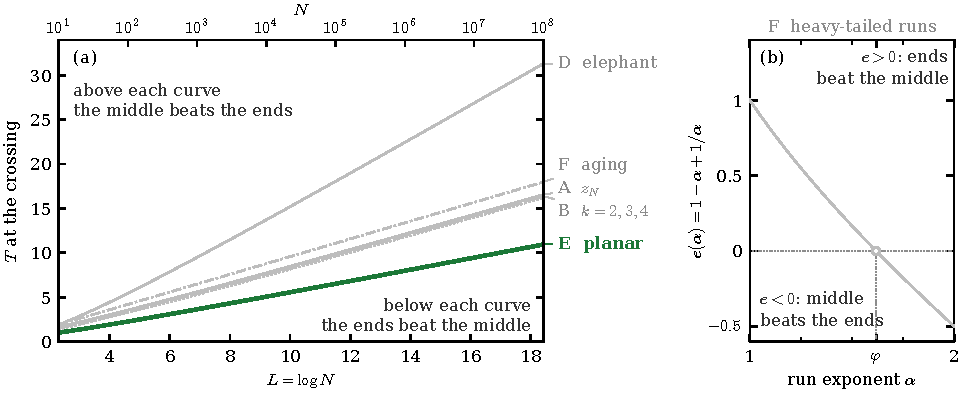
\includegraphics[width=\textwidth]{program_E}
\caption{(a) The crossing on each model's switching scale against $L=\log N$
for the papers of the series. The scale is $T$ for Papers~A, B and~E, $x=N\varepsilon$ for the
elephant walk of Paper~D and the expected number of switches for the aging walk of
Paper~F. The bold curve solves the first crossing equation of
Corollary~\ref{cor:planar-turn} for the planar walk with $r=s=1$, without its
$o(1)$ term. The curve A is $z_N$, and the curves B are the face crossings of
Paper~B.
(b) The exponent $e(\alpha)=1-\alpha+1/\alpha$ of Paper~F for runs with heavy
tails, which changes sign at the golden ratio $\varphi$. (Versions of this
figure also appear in Papers~C, D and~F.)}
\label{fig:program}
\end{figure}

\subsection{Related work}\label{sec:related}

On the lattice the correlated random walk goes back to
Gillis~\cite{gillis1955}. Chen and Renshaw~\cite{chenrenshaw1992} treat the
Gillis--Domb--Fisher walk, and in~\cite{chenrenshaw1994} they show that the
characteristic function of any correlated random walk satisfies a
recurrence. So in principle the law of our planar walk is known. Marris and
Giuggioli~\cite{marris2024} give lattice propagators for walks with forward,
backward and lateral steps. Lenci~\cite{lenci2007} proves recurrence for a
large class of persistent walks on the square lattice. In the continuum, Santra, Basu and
Sabhapandit~\cite{santra2020} find the marginals of a run-and-tumble particle
with four directions, and Angelani~\cite{angelani2022} treats switching among
four orthogonal directions. With turns only, the continuous motion is a
rotation of two independent telegraph processes (Cinque and
Orsingher~\cite[Theorem~2.2]{cinqueorsingher2023}, who credit
Orsingher~\cite{orsingher2000} for constant rates, and Smith, Le Doussal,
Majumdar and Schehr~\cite{sldms2022}). With reversals the two processes are
no longer independent~\cite[Section~3]{cinqueorsingher2023}.
Proposition~\ref{prop:product} is a lattice form of this, and on the lattice
the independent case does have reversals. In the continuum the corners carry
atoms and the origin does not (it has a density in the plane, and with
reversals also along the axes~\cite{kolesnikorsingher2002}), so the comparison
of a corner with the origin is a lattice question. We did
not find the planar crossing of the corner
and the origin in the literature.

\subsection{Plan of the paper}\label{sec:plan}

Section~\ref{sec:notation} fixes the notation and recalls what we use from Paper~A.
Section~\ref{sec:planar} treats the planar walk for general rates. It splits the origin mass,
proves the first-order answer, and locates the crossing when reversals dominate and when turns
dominate. Section~\ref{sec:product} treats the product curve and the walk with turns only.
Section~\ref{sec:verify} describes the computer checks and the open questions, and
Appendix~\ref{app:planar} has the longer proofs.
